%% LyX 2.1.1 created this file.  For more info, see http://www.lyx.org/.
%% Do not edit unless you really know what you are doing.
\documentclass[english]{llncs}
\usepackage[T1]{fontenc}
\usepackage[latin9]{inputenc}
\usepackage{color}
\usepackage{array}
\usepackage{url}
\usepackage{graphicx}
\PassOptionsToPackage{normalem}{ulem}
\usepackage{ulem}
\usepackage{algorithmic}
\usepackage{epstopdf} 
\usepackage{comment}
\usepackage{amsmath,amsfonts,amssymb}

% Define argmin, argmax
\def\argmax{\operatornamewithlimits{arg\,max}}
\def\argmin{\operatornamewithlimits{arg\,min}}
\newcommand{\subfour}[1]{\vspace*{3mm}{\noindent\bf #1}}

\makeatletter

%%%%%%%%%%%%%%%%%%%%%%%%%%%%%% LyX specific LaTeX commands.
%% Because html converters don't know tabularnewline
\providecommand{\tabularnewline}{\\}

%%%%%%%%%%%%%%%%%%%%%%%%%%%%%% User specified LaTeX commands.


\@ifundefined{showcaptionsetup}{}{%
 \PassOptionsToPackage{caption=false}{subfig}}
\usepackage{subfig}
\makeatother

\usepackage{babel}
\begin{document}
\title{A Study of Query Reformulation Methods for Patent Prior Art Search with Partial Patent Applications}
\maketitle
\begin{abstract}
Patents are used by entities to legally protect their inventions and
represent a multi-billion dollar industry of licensing and litigation.
In 2013, 302,948 patent applications were approved in the US alone --
a number that has doubled in the past 15 years and which makes prior
art search a daunting, but necessary task in the patent application
process.  In this work, we seek to investigate the efficacy of prior
art search strategies from the perspective of the inventor who wishes
to assess the patentability of their ideas prior to writing a full
application.  While much of the literature inspired by the evaluation
framework of the CLEF-IP competition has aimed to assist patent
examiners in assessing prior art for complete patent applications,
less of this work has focused on patent search with queries
representing partial applications.  In the (partial) patent search
setting, a query is often much longer than in other standard IR tasks,
e.g., a claims section may contain hundreds or even thousands of
words.  While the length of such queries may suggest query reduction
strategies to remove irrelevant terms, intentional obfuscation and
general language used in patents also suggests that it may help to
expand queries with additionally relevant terms.  To aid the patent
inventor in developing an effective pre-application prior art search
strategy, we comparatively evaluate a variety of partial application
search and query reformulation methods.  Among numerous findings,
querying with a full description in conjunction with generic
(non-patent specific) query reduction methods is recommended for best
performance.  However, we also find that querying with an abstract
represents the best trade-off in terms of writing effort vs. retrieval
efficacy (i.e., querying with the claims or description sections only
lead to marginal improvements) and that for such relatively short
queries, generic query expansion methods help.
%This has led the research to focus on query
%reformulation for patent search.  In this paper, we carry out an
%intensive study of both patent-specific and standard query
%reformulation methods for patent prior art search with partial patent
%applications.  We found that query expansion methods are useful for
%short queries (title, abstract and claims), and query reduction
%methods are often useful for medium-length sections (abstract and claims).
%We also shown that the abstract is a good section to query with,
%suggesting that writing the abstract is useful in the early stages of
%a patent drafting.

%We intend to mainly answer the following questions: \emph{What are these query reformulation methods? How do they work? What is the best section in a patent application to use as a query? What is the best query reformulation method? }

\end{abstract} 
\begin{keywords} Query Reformulation, Patent Search, Experimentation.
\end{keywords} 


\section{Introduction}

\noindent Patents are used by entities to legally protect their
inventions and represent a multi-billion dollar industry of licensing
and litigation.  In 2013, 302,948 patent applications were approved in
the US
alone\footnote{\texttt{http://www.uspto.gov/web/offices/ac/ido/oeip/taf/us\_stat.htm}},
a number that has doubled in the past 15 years.  Given that a single
existing patent may invalidate a new patent application, helping
inventors assess the patentability of an idea through a patent prior
art search before writing a complete patent application is an
important task.

Patent prior art search involves finding previously granted patents
that may be relevant to a new patent application. The objective and
challenges of standard formulations of patent prior art search are
different from those of standard text and web search
since~\cite{Magdy2012} (i) queries are (partial) patent applications,
which consist of documents with hundreds or thousands of words
organized into several sections, while typical queries in text and web
search constitute only a few words; and (ii) patent prior art search is a
recall-oriented task, where the primary focus is to retrieve all
relevant documents at early ranks, in contrast to text and web search
that are precision-oriented, where the primary goal is to retrieve a
subset of documents that satisfy the query intent.  Another important
characteristic of patent prior art search is that, in contrast to
scientific and technical writers, patent writers tend to generalize
and maximize the scope of what is protected by a patent, which further
complicates the task of formulating effective queries.

While much of the literature inspired by the evaluation framework of
the CLEF-IP competition has aimed to assist patent examiners in
assessing prior art for complete patent applications, less work has
focused on assessing the patentability of inventions before writing a
full patent application.  Furthermore, prior art search with queries
that represent unfinished patent applications is generally desirable, since
writing a full application is time-consuming and costly, especially if
lawyers are hired to assist.

%However prior art search with partial applications is much different than queries with a full application -- namely because the queries are much shorter and represent only parts of a patent application.

%NOTE: start a paragaph with the key idea%A patent application is organized in, at least, four sections: title,%abstract, claims and description. We assumed that a partial application%consist in one of the mentioned sections. 

\begin{figure}[!t]
\centering
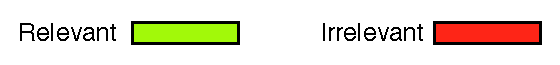
\includegraphics[width=6cm]{img/legend} 

\noindent\hspace{-5mm}\mbox{
\subfloat[Title query.]{\begin{centering}
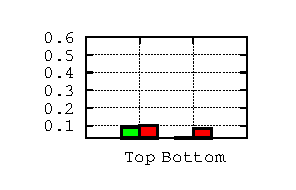
\includegraphics[width=2.9cm]{Results-CIKM2014/jaccard-qTitle-CLEF-IP2010} 
\par\end{centering}

}\subfloat[Abstract query.]{\begin{centering}
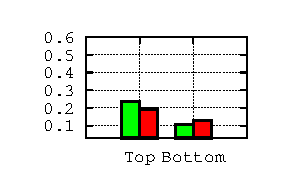
\includegraphics[width=2.9cm]{Results-CIKM2014/jaccard-qAbstract-CLEF-IP2010} 
\par\end{centering}

}\subfloat[Claims query.]{\begin{centering}
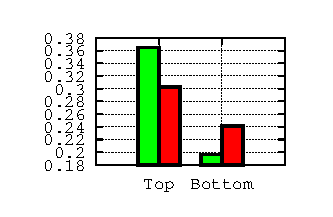
\includegraphics[width=2.9cm]{Results-CIKM2014/jaccard-qClaims-CLEF-IP2010} 
\par\end{centering}

}\subfloat[Description query.]{\begin{centering}
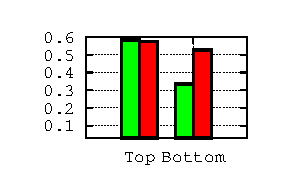
\includegraphics[width=2.9cm]{Results-CIKM2014/jaccard-qDescription-CLEF-IP2010} 
\par\end{centering}
}}

\caption{Average Jaccard similarity between fields of topics and the corresponding
(ir)relevant documents for different sets of top and bottom performing queries.}
\label{fig:FailureAnalysis}
\end{figure}


To assess the difficulty of querying with partial patent applications,
we refer to Figure~\ref{fig:FailureAnalysis}. Here we show an analysis
of the average Jaccard similarity%
\footnote{The Jaccard similarity is used to measure the term overlap between
two sets. Before applying the Jaccard similarity, patent-specific
stopwords were removed, as suggested by \cite{Mahdabi2012}.%
} between different queries (representing the title, abstract, claims,
or descriptions of partial patent applications)
and the labeled relevant (all) and irrelevant documents (top 10 irrelevant
documents ranked by BM25~\cite{Robertson1993}). We show results
for the top 100 and bottom 100 queries (100 queries that perform the
best, and 100 queries that perform the worst) of CLEP-IP 2010 evaluated
according to Mean Average Precision (MAP). Note that while the title
section is usually composed of an average of six terms, the other
sections are longer, ranging from tens to thousands of terms. There
are three notable trends here: (i) term overlap increases from title
to description since the query size grows accordingly; (ii) the bottom
100 performing queries tend to have much smaller term overlap with
the relevant documents than the top 100 queries; and (iii) even in the
best case of querying with very long description sections, the average term 
overlap indicates many terms of relevant documents are not found in the query.

%**Highly redundant with above content**
%
%While these results suggest the description section is the best part
%of a partial patent application to use as query, they also point out
%that the term overlap between the queries and the relevant documents
%can be very low. Also, in this context, a query is much longer than
%in other standard IR tasks. It can take the form of a long paragraph
%(e.g. the case of the abstract used for querying), or even a very
%long document (e.g. the case of claims or the description used for
%querying). 
Similar observations in the general patent prior art search
literature~\cite{Magdy2011} have led to a research focus on query
reformulation.  Therefore, we suggest an
investigation of \emph{query reformulation}~\cite{Baeza-Yates2010}
methods as a means for improving the term overlap between queries that
represent partial patent applications and relevant documents, with the
objective of assessing not only the performance of standard query
reformulation methods, but also the effectiveness of query
reformulation methods that exploit patent-specific characteristics. 

In summary, to aid the patent inventor in developing an effective
pre-application prior art search strategy, we seek to answer the
following questions in this work:
\begin{itemize}
\item What parts of a patent application should a patent inventor
write first to achieve effective prior art search?  What
are the trade-offs in section writing effort vs. the retrieval
performance of querying with that section?
\item In query expansion, do any sections of patents serve as better
sources of expansion terms?  What expansion methods work best, and in what settings?
\item For query reformulation (both query expansion and reduction),
which methods work best, and in what settings?  Do patent-specific
reformulation methods offer advantages over more generic IR reformulation
methods?
\end{itemize}
To answer these questions, we perform a thorough comparative analysis
of partial patent application query strategies and reformulation methods on
the CLEF-IP patent prior art search datasets.

The rest of the paper is organized as follows: in
Section~\ref{sec:QueryReformulation}, we present a variety of generic
and patent-specific query reformulation methods; in
Section~\ref{sec:Evaluation}, we present the evaluation results and
analysis to answer the above questions; and in
Section~\ref{sec:Conclusion}, we conclude with key observations from
this evaluation that lead to concrete recommendations for 
patent prior art search with partial applications.


\section{Query Reformulation for Patents}

\label{sec:QueryReformulation}

Query Reformulation is the process of transforming an initial query
$Q$ to another query $Q'$. This transformation may be either an
expansion or a reduction of the query.\emph{ Query Expansion} (QE)
\cite{Efthimiadis1996} enhances the query with additional terms likely
to occur in relevant documents. Hence, given a query representation
$Q$, QE aims to select an optimal subset $T_{k}$ of $k$ terms,
which are relevant to $Q$, then build $Q'$ such as $Q'=Q\cup T_{k}$.
As for \emph{Query Reduction} (QR) \cite{Kumaran2009}, it is the
process that reduces the query such that superfluous information is
removed. Hence, given a query representation $Q$, QR aims to select
an optimal subset $T_{k}\subset Q$ of $k$ terms, which are relevant
to $Q$, then build $Q'$ such as $Q'=T_{k}$.

In the following sections, we describe the standard and patent-specific 
query reformulation methods that we evaluate in Section~\ref{sec:Evaluation}.


\subsection{Standard Query Reformulation Methods}
\label{sec:StandardQRMethods}


\subfour{The Rocchio Algorithm for Relevance Feedback:}
The Rocchio algorithm \cite{Salton1971} is a classic algorithm of
relevance feedback used mainly for query expansion.  In brief, it
provides a method of incorporating relevance feedback information into
the vector space model representing a query \cite{Manning2008}. The
underlying theory behind Rocchio is to find a query vector
$\overrightarrow{Q'}$, that maximizes similarity with relevant
documents while minimizing similarity with irrelevant
documents. Typically, a pseudo-relevance feedback (PRF) set of $k$ top
ranked documents obtained after an initial run of the query is
considered as the set of relevant documents to build
$\overrightarrow{Q'}$. We refer to this method as RocchioQE.%
\footnote{We used the LucQE module, which provides an implementation of the
Rocchio method for Lucene. \texttt{http://lucene-qe.sourceforge.net/}%
}

Similarly, Rocchio can be used as a QR method.  Basically, the idea is
that once the Rocchio-modified query vector has been computed, it is
possible to select only the terms that appear in the initial query $Q$
and rank them using the Rocchio score and finally, select the top $k$
terms with the highest score to build $Q'$. We refer to this approach
as RocchioQR.


\subfour{Maximal Marginal Relevance for Query Reformulation:}
As a general method for query reformulation, we also consider a method
of ``diverse'' term selection --- an adaptation of the \emph{Maximal
  Marginal Relevance} (MMR)~\cite{Carbonell1998} algorithm for result
set diversification.  But, rather than use MMR for diverse document
selection (as typically used), it is used here for diverse term
selection --- the hypothesis being that diverse term selection may
improve coverage of relevant terms in the PRF set.

%The idea is to use MMR for diverse term selection. 
%\subfour{MMR Query Expansion (MMRQE)}
%\label{sec:MMRQE}

%%%%%%%%%%%%%%%%%%%%%%%%%%%%%%%%%%%%%%%%%%%%%%%%%%%%%%%%%%%%%%%%%%%%%
\begin{figure}[!t]
\begin{centering}
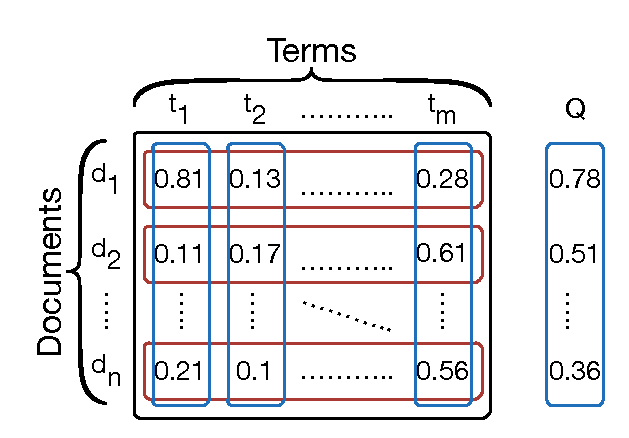
\includegraphics[width=5cm]{img/matrix} 
\par\end{centering}
\protect\caption{Notation used in MMR QE/QR.}
\label{fig:Notation} 
\end{figure}
 
%%%%%%%%%%%%%%%%%%%%%%%%%%%%%%%%%%%%%%%%%%%%%%%%%%%%%%%%%%%%%%%%%%%%%

In the case of QE, we call this diversified expansion method MMR Query Expansion
(MMRQE). MMRQE takes as input a PRF set, which is used to build a
document-term matrix of $n$ documents and $m$ terms as shown in
Figure~\ref{fig:Notation} (the TF-IDF is used to populate the matrix
for each document vector). To represent the query $Q$ in the documents'
dimension as in Figure~\ref{fig:Notation}, we use the BM25 or TF-IDF
score between each document $d_{i}$ and the query. Hence, given a
query representation $Q$, MMRQE aims to select an optimal subset
of $k$ terms $T_{k}^{*}\subset D$ (where $|T_{k}^{*}|=k$ and $k\ll|m|$)
relevant to $Q$ but inherently different from each other (i.e., diverse).
This can be achieved by building $T_{k}^{*}$ in a greedy manner by
choosing the next optimal term $t_{k}^{*}$ given the previous set
of optimal term selections $T_{k-1}^{*}=\{t_{1}^{*},\ldots,t_{k-1}^{*}\}$
(assuming $T_{0}^{*}=\emptyset$) using the MMR diverse selection
criterion:

\begin{equation}
t_{k}^{*}=\argmax_{t_{k}\notin T_{k-1}^{*}}\hspace{-0.3mm}[\lambda\cos(Q,t_{k})-\hspace{-0.3mm}(1-\lambda)\max_{t_{j}\in T_{k-1}^{*}}\cos(t_{j},t_{k})]\label{eq:MMRQE-QR}
\end{equation}

Here, the first cosine similarity term measures relevance between
the query $Q$ and possible expansion term $t_{k}$ while the second
term penalizes the possible expansion term according to it is cosine
similarity with any currently selected term in $T_{k-1}^{*}$. The
parameter $\lambda\in[0,1]$ trades off relevance and diversity.
For MMRQE, we found that $\lambda=0.5$ generally provide the best results, according to our experiments on the CLEF-IP training dataset collection.

For QR, we can greedily rebuild the query from scratch,
while choosing diversified terms from the query itself.  Here,
we call this approach MMR Query Reduction (MMRQR). Formally, given
a query representation $Q$, MMRQR aims to select an optimal subset
of $k$ terms $T_{k}^{*}\subset Q$ (where $|T_{k}^{*}|=k$ and $k<|Q|$)
relevant to $Q$ but inherently different from each other (i.e., diverse).
This can be achieved by building $T_{k}^{*}$ in a greedy manner by
choosing the next optimal term $t_{k}^{*}$ given the previous set
of optimal term selections $T_{k-1}^{*}=\{t_{1}^{*},\ldots,t_{k-1}^{*}\}$
(assuming $T_{0}^{*}=\emptyset$) using an adaptation of the MMR diverse
selection criterion. Note that we use all the sections of the
patent documents in the PRF set to built the document-term matrix
of $n$ documents and $m$ terms shown in Figure~\ref{fig:Notation}.
For MMRQR, we found that $\lambda=0.8$ generally provide the best results in our experiments on the CLEF-IP dataset collection.

The key insight we want to highlight is that MMRQE
does not select expansion terms independently as in practical usage
of Rocchio, but rather it selects terms that have uncorrelated usage
patterns across documents, thus hopefully encouraging diverse term
selection that covers more documents for a fixed expansion budget
$k$ and ideally, higher recall.

\subsection{Patent-specific Query Reformulation Methods}
\label{sec:SpecificQRMethods}

%In this section, we first describe two patent-specific query expansionmethods, then, we describe two patent-specific query reduction methods.

\subfour{Synonym Sets for Patent Query Expansion:}
Magdy et al. \cite{Magdy2011} proposed a patent query expansion method,
which automatically generates candidate synonym sets (SynSet) for
terms to use as a source of expansion terms. The idea for generating
the SynSet comes from the characteristics of the CLEF-IP patent collection,
where some of the sections in some patents are translated into three
languages (English, French, and German). They used these parallel
manual translations to create possible synonyms sets. Hence, for a
word $w$ in one language which has possible translations to a set
of words in another language ${w_{1},w_{2},\ldots,w_{n}}$, this set
of words can be considered as synonyms or at least related to each
other. The generated SynSet is used for query expansion in two ways:
(i) The first one used the probability associated with the SynSet entries
as a weight for each expanded term in the query (denoted WSynSet).
Therefore, each term was replaced with its SynSet entries with the
probability of each item in the SynSet acting as a weight to the term
within the query. (ii) The second one neglected this associated probability
and used uniform weighting for all synonyms of a given term (denoted
USynSet).


\subfour{Patent Lexicon for Query Expansion:}
Mahdabi et al. \cite{Mahdabi2013} proposed to build a query-specific
patent lexicon based on definitions of the International Patent Classification
(IPC). The lexicon is simply built by removing general and patent-specific 
stop-words from the text of IPC definition pages.  Each entry in the
lexicon is composed of a key and a value. The key is an IPC class
and the value is a set of terms representing the mentioned class.
Then, the lexicon is used to extract expansion concepts related
to the context of the information need of a given query patent. To
this end, the IPC class of the query patent is searched in the lexicon
and the terms matching this class are considered as candidate expansion
terms. The proposed approach tries to combine these two complementary
vocabularies. In this paper we refer to this patent query expansion
method as IPC Codes.


\subfour{Language Model for Query Reduction:}
In \cite{Ganguly2011}, the authors proposed a query reduction technique,
which decomposes a query (a patent section) into constituent text
segments and computes Language Model (LM) similarities by calculating
the probability of generating each segment from the top ranked documents
(PRF set). Then, the query is reduced by removing the least similar
segments from the query. We refer to this method as LMQR.


\subfour{IPC Codes for Query Reduction:}
Based on the intuition that, terms in the IPC code definition may
represent \textquotedbl{}stop-words\textquotedbl{}, especially if they
are rare (infrequent in the patent application), one can think to
reduce a patent query as follows: (i) For each patent application,
take the definitions of the IPC codes which are associated to it.
Then, (ii) rank the terms of the query according to the difference in
their frequency in the query and their frequency in the class code
definition. Finally, (iii) remove bottom terms of this ranking from
the query (i.e. good terms are terms that occur a lot in the query,
and few in the class code definition, whereas bad terms are those that
occur few in the query, and a lot in the class code definition). In
the evaluation section we denote this approach IPC-StopWords.

%%
%% Reviewers may point out that we should have compared...
%%
\subfour{Further Afield:}
While some more complex patent-specific methods have also been
explored for general patent prior art
search~\cite{Bashir2010,Verma2011,Mahdabi2013}, space limitations
preclude an exhaustive comparison to all available methods.
Notwithstanding this, we believe the above outlined patent-specific
query reformulation methods circumscribe a range of patent-specific
approaches spanning synonym lexicons, specially derived language
models, and IPC code resources; hence our evaluation supports the
objective of identifying general query reformulation methods from the
novel perspective of partial patent application prior art search that
may be deserving of further investigation in future work.

%we do
%do not show comparisons with these methods here for the following reasons:
%(i) their authors already pointed out their poor performance \cite{Mahdabi2013}; 
%(ii) as reflected in our existing experiments, patent-specific lexicons
%have not tended to yield significantly better query reformulation results
%in comparison to generic methods~\cite{Magdy2011,Verma2011}; and 
%(iii) the method is computational too expensive \cite{Bashir2010}.


\section{Experimental Evaluation}
\label{sec:Evaluation}

In this section we first explain the experimental setup for evaluating
the effectiveness of patent prior art search with partial applications. Then,
we discuss the results of QE and QR methods in Sections~\ref{sec:QEResults}
and~\ref{sec:QRResults} respectively.


\subsection{Experimental Setup}
\label{sec:Setup}

For our experiments, we used used the Lucene IR System%
\footnote{\texttt{http://lucene.apache.org/}%
} to index the English subset of CLEF-IP 2010 and CLEF-IP 2011 datasets%
\footnote{\texttt{\url{http://www.ifs.tuwien.ac.at/~clef-ip/}}%
}~\cite{Piroi2011,Roda2009} with the default settings for stemming and stop-word
removal. We also removed patent-specific stop-words as described in
\cite{Magdy2012}.  CLEF-IP 2010 contains 2.6 million patent documents,
and the English test sets of CLEF-IP 2010 correspond to 1303 topic
sources of partial patent application queries.  We also experimented
with the CLEF-IP 2011 dataset, but observed the same overall trends as
for CLEF-IP 2010 and hence omit these redundant results due to space
limitations.

In our implementation, each section of a patent (title, abstract,
claims, and description) is indexed in a separate field so that different
sections can be used, for example, as source of expansion terms.  However,
when a query is processed, all indexed fields are targeted, since this
generally offers best retrieval performance.
As suggested in previous work~\cite{Lopez2009,Roda2009} and found to yield
best results in our experiments, we used the patent classification (IPC) 
codes assigned to the query topics to filter search results to match
at least one of the query IPC codes.

We report both MAP and PRES (Patent Retrieval Evaluation Score). The
PRES metric places more emphasis on high-recall retrieval by weighting
relevant documents lower in the ranking more highly than MAP.  We
report these ranking evaluation metrics on the top 1000 results.

\subsection{Query Expansion Results}

\label{sec:QEResults}

In this section, we discuss the results of partial patent queries
with the QE methods described in Section \ref{sec:QueryReformulation}.
In doing this experimentation, there are many configuration options and 
associated questions to consider: 

\begin{itemize}
\item \textbf{Partial patent query type:} We consider a query of
  a partial patent application to consist of either the title, the
  abstract, the claims, or the description section. Critical questions
  are: what part of a partial application an inventor should write to
  obtain the best search results?  And what QE methods work best for
  each type of query?
\item \textbf{Query expansion source:} We consider the abstract,
  claims, and description sections as different term sources to
  determine which section offers the best source of expansion terms,
  e.g., are words in the claims of particularly high value as
  expansion terms?  We omit the use of the title as a source
  of expansion terms noting that this
  configuration performed poorly due to the relative sparsity of
  useful expansion terms in the titles of the PRF set.
\item \textbf{Relevance model:} For initial retrieval of documents in
  the \emph{pseudo-relevant} feedback set (PRF) and subsequent
  re-retrieval, there are various options for the relevance ranking
  model. In this work, we explore a probabilistic approach represented
  by the popular BM25~\cite{Robertson1993} algorithm, as well as a
  vector space model (VSM) approach, TF-IDF~\cite{Salton1975}. A
  natural question is which relevance model works best for query
  expansion for patent prior art search?
\item \textbf{Term selection method:} We consider the different query
  expansion methods described above, i.e. RocchioQE, MMRQE, IPC Codes,
  WSynSet, USynSet and ask what is the best QE method for patent search?
\end{itemize}


%%%%%%%%%%%%%%%%%%%%%%%%%%%%%%%%%%%%%%%%%%%%%%%%%%%%%%%%%%%%%%%%%%%
\begin{figure*}[tb]
\begin{centering}
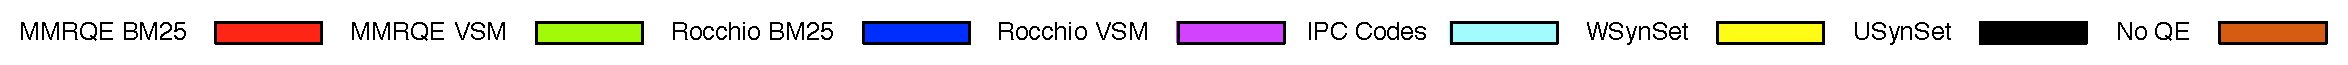
\includegraphics[width=12cm]{img/legendQE} 
\par\end{centering}

\begin{centering}
\subfloat[Query Title.]{\begin{centering}
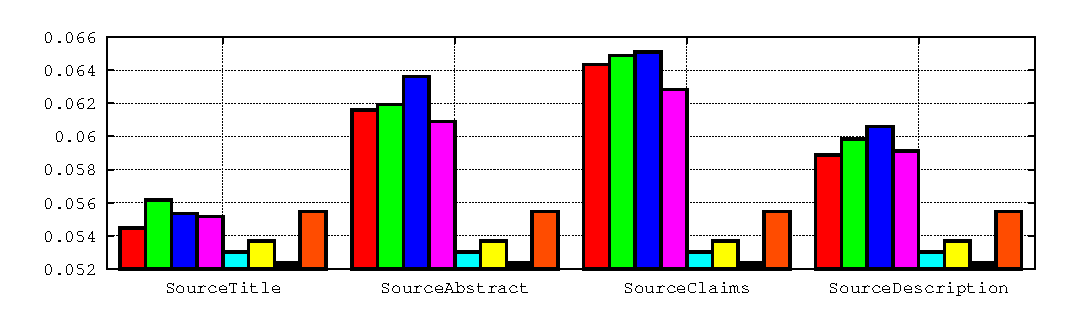
\includegraphics[width=6cm]{Results-CIKM2014/qTitle-MAP-CLEF-IP2010} 
\par\end{centering}

}\subfloat[Query Abstract.]{\begin{centering}
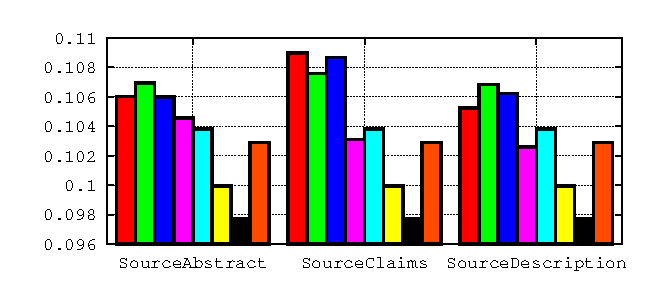
\includegraphics[width=6cm]{Results-CIKM2014/qAbstract-MAP-CLEF-IP2010} 
\par\end{centering}

}
\par\end{centering}

\begin{centering}
\subfloat[Query Claims.]{\begin{centering}
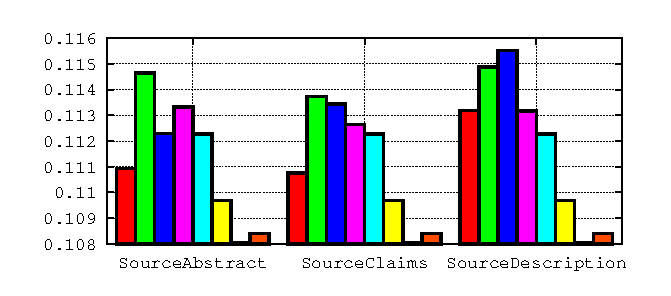
\includegraphics[width=6cm]{Results-CIKM2014/qClaims-MAP-CLEF-IP2010} 
\par\end{centering}

}\subfloat[Query Description.]{\begin{centering}
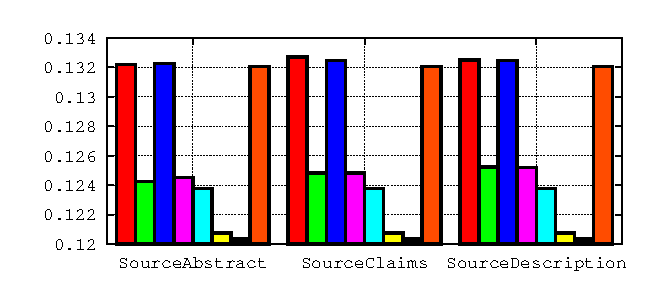
\includegraphics[width=6cm]{Results-CIKM2014/qDescription-MAP-CLEF-IP2010} 
\par\end{centering}

\label{fig:qDescription-MAP-CLEF-IP2010}}
\par\end{centering}

\protect\caption{MAP for QE methods on CLEF-IP 2010.}
\label{fig:MAP-CLEF2010} 
\end{figure*}
%%%%%%%%%%%%%%%%%%%%%%%%%%%%%%%%%%%%%%%%%%%%%%%%%%%%%%%%%%%%%%%%%%%

%%%%%%%%%%%%%%%%%%%%%%%%%%%%%%%%%%%%%%%%%%%%%%%%%%%%%%%%%%%%%%%%%%%
\begin{figure*}[tb]
\begin{centering}
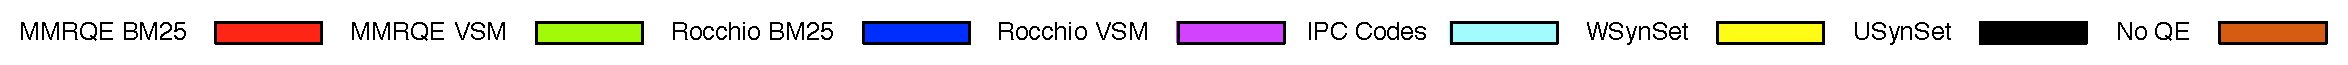
\includegraphics[width=12cm]{img/legendQE} 
\par\end{centering}

\begin{centering}
\subfloat[Query Title.]{\begin{centering}
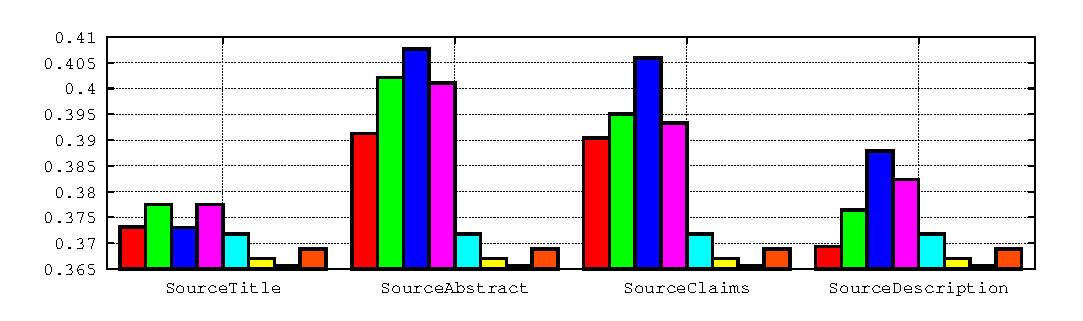
\includegraphics[width=6cm]{Results-CIKM2014/qTitle-PRES-CLEF-IP2010} 
\par\end{centering}

}\subfloat[Query Abstract.]{\begin{centering}
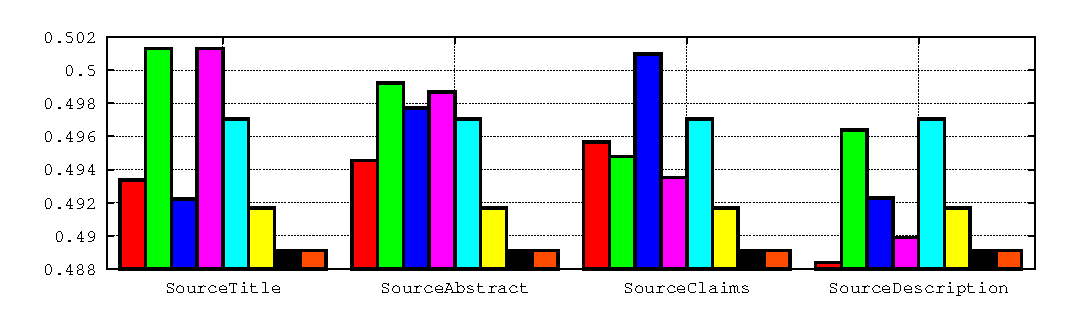
\includegraphics[width=6cm]{Results-CIKM2014/qAbstract-PRES-CLEF-IP2010} 
\par\end{centering}

}
\par\end{centering}

\begin{centering}
\subfloat[Query Claims.]{\begin{centering}
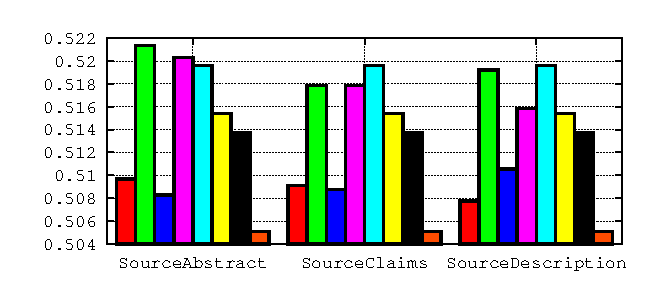
\includegraphics[width=6cm]{Results-CIKM2014/qClaims-PRES-CLEF-IP2010} 
\par\end{centering}

}\subfloat[Query Description.]{\begin{centering}
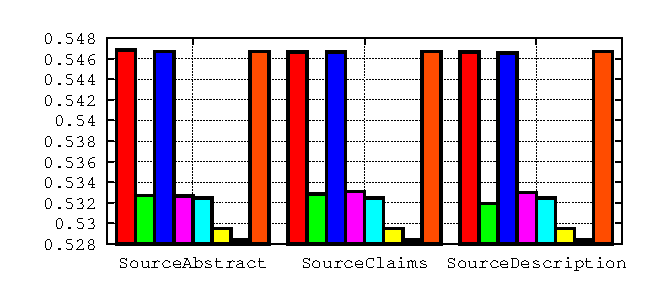
\includegraphics[width=6cm]{Results-CIKM2014/qDescription-PRES-CLEF-IP2010} 
\par\end{centering}

\label{fig:qDescription-PRES-CLEF-IP2010}}
\par\end{centering}

\protect\caption{PRES for QE methods on CLEF-IP 2010.}
\label{fig:PRES-CLEF2010} 
\end{figure*}
%%%%%%%%%%%%%%%%%%%%%%%%%%%%%%%%%%%%%%%%%%%%%%%%%%%%%%%%%%%%%%%%%%%

To summarize all the results obtained over all the above
configurations, Figure \ref{fig:MAP-CLEF2010} and Figure
\ref{fig:PRES-CLEF2010} shows the MAP and PRES obtained for all the QE
methods, while selecting the optimal number of terms used for the
expansion (the number of terms that maximizes the performance for each
method). From these results, we make the following observations:

\begin{enumerate}
\item The best partial application section to use for querying is the
  description section. %(see Figure \ref{fig:qDescription-PRES-CLEF-IP2010}). 
  We attribute this to the
  fact that the description section has more content along with
  relevant terms that define the invention since a detailed summary of
  the invention is described therein. 
 \item However, perhaps a better trade-off in terms of effort
   vs. retrieval performance is to query with the abstract.  Relative
   to the description, it takes much less effort to write the abstract.
   Further, querying with the abstract provides a substantial boost in
   retrieval performance compared to the title (about 165\%).  
   In contrast, querying
   with the claims and description offer only marginal performance gains
   (about 10\% to 30\% for MAP) compared to using the abstract.
\item Query expansion is not useful for very long queries
  (i.e. description) since no method outperforms the baseline. This
  indicates that in advanced writing stages of the patent preparation process,
  QE is not useful.% (see Figure
  %\ref{fig:qDescription-MAP-CLEF-IP2010} and Figure
  %\ref{fig:qDescription-PRES-CLEF-IP2010}).
\item When dealing with short queries such as the title or abstract, 
  MMRQE is less effective than Rocchio, whereas it appears to provide
  slightly better comparative results for the longer claims query.  This suggests 
  diverse term selection may be helpful for long queries.
%% I don't think the results clearly support the following statements...
%% just omit since they aren't crucial for the paper.  -Scott
%%
%\item The best source for query expansion is the claims section. We
%  attribute this to the fact that, the claims contain not only
%  relevant, but also, specific terminology, since the scope of the
%  invention is described therein. However, when querying using the
%  claims, other sources of query expansion provided better
%  performance. This may be because claims are very similar between
%  them and contained specific terms; consequently, the queries lack of
%  diversity and general terms or synonyms that are used to describe
%  similar inventions.
\item The description section does not appear to be a good source for
  expansion, likely since its content is too broad and it contains  
  many irrelevant terms.
\item In general, generic QE methods like Rocchio tend to outperform
  patent-specific QE methods, although among patent-specific methods,
  SynSet approaches seemed to work best.
%\item Using the IPC code definitions (as suggested by
%  \cite{Mahdabi2013}) and SynSet (method of \cite{Magdy2011}) as a
%  source of expansion, gave poor performance (see IPC Codes and SynSet
%  bars along the Figures).
%\item Finally, regarding the best term selection method, we conclude
%  that in general, MMRQE provides the best performance, followed by
%  RocchioQE.
\end{enumerate}

%To give an insight of the effect of MMRQE and Rocchio over the performance, Table \ref{tbl:QESampleQueries} shows two queries where QE methods improved the performance. First of all, it is interesting to notice that even if there are common terms selected to expand the queries by both MMRQE and Rocchio, the lists of MMRQE contain more diversified terms (at least in the first example). For the first example, relevant patents talk about a similar idea than the application, but using different complex and ambiguous terms. Hence, for the first query, key terms  like: \textit{rotor, blend, and suction}, were able to capture the scope of the relevant patents to allow either retrieving them (improving PRES), or pushing them to the top of the ranking (improving MAP). As for the second query, MMRQE expand the query with general terms, e.g. \textit{result, includ, extend, plural}, which probably encourage retrieving irrelevant patents.


%%%%%%%%%%%%%%%%%%%%%%%%%%%%%%%%%%%%%%%%%%%%%%%%%%%%%%%%%%%%%%%%%%%
\begin{figure*}[tb]
\begin{centering}
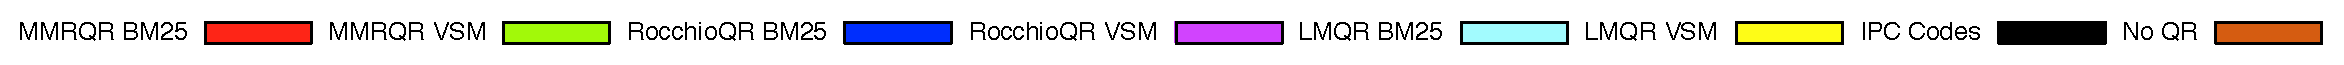
\includegraphics[width=12cm]{img/legendQR} 
\par\end{centering}

\begin{centering}
\subfloat[Query Abstract.]{\begin{centering}
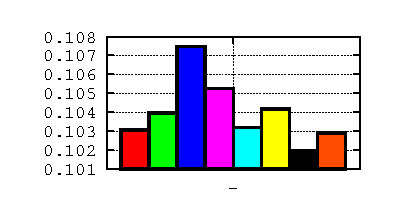
\includegraphics[width=4cm]{mmrqrResults/qAbstract-MAP-CLEF-IP2010} 
\par\end{centering}

}\subfloat[Query Claims.]{\begin{centering}
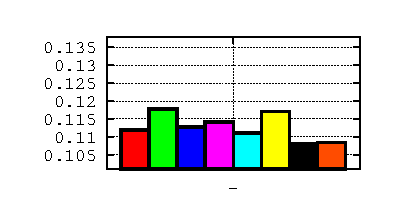
\includegraphics[width=4cm]{mmrqrResults/qClaims-MAP-CLEF-IP2010} 
\par\end{centering}

}\subfloat[Query Description.]{\begin{centering}
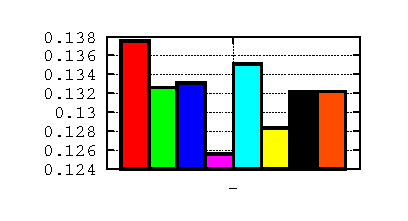
\includegraphics[width=4cm]{mmrqrResults/qDescription-MAP-CLEF-IP2010} 
\par\end{centering}

}
\par\end{centering}

\protect\caption{MAP for QR methods on CLEF-IP 2010.}
\label{fig:QR-MAP-CLEF-IP2010}
\end{figure*}
%%%%%%%%%%%%%%%%%%%%%%%%%%%%%%%%%%%%%%%%%%%%%%%%%%%%%%%%%%%%%%%%%%%

%%%%%%%%%%%%%%%%%%%%%%%%%%%%%%%%%%%%%%%%%%%%%%%%%%%%%%%%%%%%%%%%%%%
\begin{figure*}[tb]
\begin{centering}
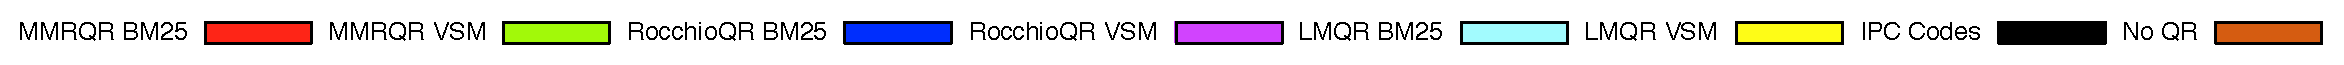
\includegraphics[width=12cm]{img/legendQR} 
\par\end{centering}

\begin{centering}
\subfloat[Query Abstract.]{\begin{centering}
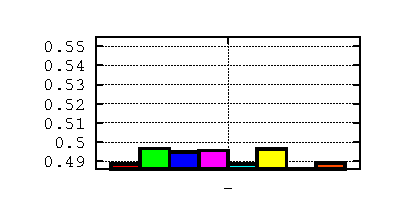
\includegraphics[width=4cm]{mmrqrResults/qAbstract-PRES-CLEF-IP2010} 
\par\end{centering}

}\subfloat[Query Claims.]{\begin{centering}
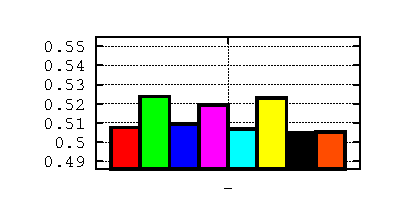
\includegraphics[width=4cm]{mmrqrResults/qClaims-PRES-CLEF-IP2010} 
\par\end{centering}

}\subfloat[Query Description.]{\begin{centering}
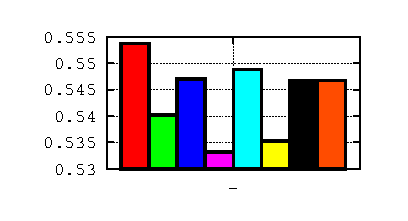
\includegraphics[width=4cm]{mmrqrResults/qDescription-PRES-CLEF-IP2010} 
\par\end{centering}

}
\par\end{centering}
\protect\caption{PRES for QR methods on CLEF 2010.}

\label{fig:QR-PRES-CLEF-IP2011} 
\end{figure*}
%%%%%%%%%%%%%%%%%%%%%%%%%%%%%%%%%%%%%%%%%%%%%%%%%%%%%%%%%%%%%%%%%%%

\subsection{Query Reduction Results}

\label{sec:QRResults}

Next we discuss the results of the evaluation performed
on the QR methods described in Section \ref{sec:QueryReformulation}.
As for QE, we carry out comprehensive experiments with the following
configuration options and associated questions to consider: 

\begin{itemize}
\item \textbf{Partial patent query type:} We apply QR methods to a
  query of a partial patent application, consisting of the abstract,
  the claims or the description sections. A critical question is what
  part of a partial application is best suited for QR?  Note that we
  consider that there is no interest in reducing a title query since
  it already contains very few terms.
\item \textbf{Relevance model:} We explore a probabilistic approach
  represented by the popular BM25~\cite{Robertson1993} algorithm, as
  well as a vector space model (VSM) approach,
  TF-IDF~\cite{Salton1975}. A natural question is which relevance
  model works best for query reduction for patent prior art search?
\item \textbf{Term selection method:} We consider the different query
  reduction methods described above, i.e. RocchioQR, MMRQR, LMQR,
  IPC-StopWords and ask what is the best QR method for patent search?
  Further, how do these results compare to QE for the same queries?
\end{itemize}

To summarize all the results obtained over all the above
configurations, Figures \ref{fig:QR-MAP-CLEF-IP2010}, and
\ref{fig:QR-PRES-CLEF-IP2011} show the respective MAP and PRES
performance obtained for all QR methods, when selecting the
optimal number of terms removed from the original queries. 
From these results, we make the following
observations:

\begin{enumerate}
\item The best performing QR methods show benefits vs. No QR for all
  queries (i.e., abstract, claims, and description).
\item The term selection methods that provide the best performance
  are, in general, RocchioQR and MMRQR.
\item When dealing with medium-length queries (i.e., abstract and
  claims), VSM performs better than BM25, while for very long queries
  (i.e., description), BM25-based QR methods perform better than
  VSM-based QR methods.
\item In comparison to the corresponding MAP and PRES results
  for QE from Figure \ref{fig:MAP-CLEF2010} and Figure
  \ref{fig:PRES-CLEF2010}, the best QE and QR methods perform comparably
  for abstract and claims queries, whereas for description queries, the best QR 
  method slightly outperforms the best QE method.  Hence, the best
  overall retrieval result in this work in terms of both MAP and PRES
  comes from a description query with a generic (non-patent specific) QR method.
\end{enumerate}

\section{Conclusions}
\label{sec:Conclusion}

In this paper, we analyzed various query strategies for patent prior
art search with partial (incomplete) applications along with generic
and patent-specific query reformulation (expansion and reduction)
methods.  We performed a comprehensive comparative evaluation of these
methods on the CLEF-IP patent retrieval corpus.

We showed that the description is the best partial application section
to query with, followed by the claims, the abstract, and lastly the
title section.  However, the largest boost in performance (about 165\%
for MAP) comes when switching from a title query to an abstract query;
smaller relative boosts are given by querying instead with the claims
or description (about 10\% to 30\% for MAP).  This is a critical
insight since it is substantially easier for the patent inventor to
draft an abstract rather than a full patent description and in doing
so, still manage to retrieve the majority of prior art that would have
been retrieved with the full description.

We observed that query expansion (QE) methods are useful for short to
medium length queries (i.e., title, abstract, and claims), but useless for
very long queries (i.e., the description section).  We also showed that
the description section does not provide the best source of expansion
terms for QE, rather the claims or the abstract tend to offer better
candidate terms for QE.  In the same vein, we also found traditional
IR methods like Rocchio or variations to work just as well for QE (and
generally better) in comparison to patent-specific methods using
specialized expansion sources such as synonym lexicons or IPC code definitions.
%For QE, future work should investigate how can we exploit patent-specific
%meta-data such as inventor and citation networks to better exploit
%specialized domains of discourse relevant to patent subfields.

Regarding query reduction (QR) methods, we showed that these
techniques are generally most effective in comparison to QE for the
description section (the longest section used as a partial application
query).  Indeed, the best overall retrieval performance results in this work are
achieved with generic (non-patent specific) QR methods for a description query.

%Finally, it is clear that for a patent examiner, using the description
%section of a patent application with perhaps a QR method like MMRQR
%or RocchioQR will help to find the most relevant documents (to invalidate
%the application). However, for inventors, before investing too much
%time in writing a full patent application, we believe that it is better
%to first write the abstract. Then, use Rocchio with expanded terms coming from
%the claims to get the most relevant documents to make a prior art
%search task (to position the current invention with related work).
%
%These observations does not contradict with the  

In conclusion, returning to our initial objective to aid the patent
inventor in developing an effective pre-application prior art search
strategy, our evaluation reveals that while querying with a
full description in conjunction with generic (non-patent specific)
query reduction methods yields best overall retrieval performance, querying with
just an abstract in conjunction with generic QE methods may yield the best
trade-off in terms of writing effort vs. retrieval performance.
%Future work should investigate whether QE methods for abstract queries
%can rival the best methods for description queries --- if such a result
%were possible, it would significantly reduce the effort required on
%behalf of the patent inventor to identify potentially invalidating
%prior art for a new patent idea.

{\scriptsize{} \bibliographystyle{abbrv}
\bibliography{biblio}
}
\end{document}
